\chapter{Introduction}
\section{Introduction}


\pagenumbering{arabic}
\vspace{12pt}

 
					
The growing popularity of mobile devices such as tablets and smartphones in the modern era Google(2019 ,Aug) mobileplanet www.thinkwithgoogle.com/mobileplanet\cite{ThinkwithGoogle}, combined with their ability to support multiple network interfaces and communication protocols, has brought forth new research and development opportunities.

\vspace{12pt} 

As Smartphone usage become increasingly popular, we have a high density of mobile devices throughout most of the common areas. Data from our previous analysis support this as well. Most of these devices functionalities critically depend on the internet connection they process. Therefore there is a need for high bandwidth low-cost data connection.

\vspace{12pt} 

These days the mobile devices have become very sophisticated devices. They possess multiple network interfaces with considerable processing power. But it only uses one network interface at a time. This research is about using that underutilized interface to build an ad-hoc mesh network which will promote local routing. By doing so it will provide a cheap high bandwidth low latency connection using the readily available resources in those mobile devices.


\vspace{12pt}

\clearpage

\section{Motivation}


\pagenumbering{arabic}
\vspace{12pt}

	 Even though the current mobile devices are heavily reliant on the data connection to function they underutilize the network resources available to them. This is shown in the Cisco(2017)Global Mobile Data Traffic Forecast Update, 2017 to 2022\cite{mobile_web_penetration} Eg: If we need to transfer the file to a friend we need to do so using a data connection rather than transferring them peer to peer using wifi.
Even To communicate with multiple people in the same room there should be a cellular connection. But they are in the communication range of each other. If there was a direct connection between two devices we can achieve much higher bandwidth without any additional charge. With the local routing, we can have a redundant connection between devices. This can be very helpful for a situation where there is bad reception. If the cellular connection breaks there is a path through the ad hoc network.
So our motivation is to reduce the cost of the data connection while increasing the quality using the readily available resources of the mobile devices.
\vspace{12pt}

\section{Research significance}
\vspace{12pt}
Short-range wifi communication offers higher data transfer rates. As the white paper about wifi 802.11ax standard by (Cisco,2019).\cite{wifi-speed}suggests, we can get up to 4.8 Gbps of max data rate by this wifi standard. 
As we try to route the data locally users will get a faster internet connection without any additional infrastructure cost. And we can also reduce the cellular charges of the user significantly.
By implementing this kind of hybrid cellular-ad-hoc network we get additional high bandwidth without any additional cost to the user.


\vspace{12pt}


\vspace{12pt}





\pagebreak
\section{Background}
\pagenumbering{arabic}
\vspace{12pt}


\vspace{12pt}


\subsection{A peer-to-peer (P2P) network }
\vspace{12pt}

 According to (Schollmeier,2001)\cite{define_P_to_p} peer-to-peer network is a network of interconnected nodes ("peers") serving resources amongst each other without the use of a centralized administrative system.


\vspace{12pt}
\subsection{What is ad-hoc network}




\vspace{12pt}

According to Toh, C. (2002). Ad hoc wireless networks: Protocols and systems.  \cite{book_adhoc} an ad hoc network is a network that is comprised of individual devices interacting with each other directly. The term(ad-hoc) implies spontaneous or impromptu construction because these networks often bypass the central access point such as a router. Many ad hoc networks are local area networks where devices are enabled to send data directly to one another rather than going through a centralized access point.


\vspace{12pt}

\subsection{Mobile ad-hoc network:(MANET)}
\vspace{12pt}

According to Toh, C. (1997). Wireless ATM and ad-hoc networks: Protocols and architectures.\cite{book}These are wireless ad-hoc-networks which can self-configure dynamically to create a wireless mesh network. Nodes of this network can move freely so they have the ability to make and break the connection on the fly.


\vspace{12pt}
\subsection{What is wifi direct?}



\vspace{12pt}
According to Wi-Fi Alliance(2019,Aug) www.wi-fi.org/discover-wi-fi/wi-fi-direct \cite{WiFiDirect-by-wifi-aliance}, Wi-Fi Direct is a Wi-Fi communication standard that facilitates device connections without requiring a wireless access point (WAP). The devices are connected using Wi-Fi, thus achieving Wi-Fi level connection and transfer speeds from the connectivity.

\vspace{12pt}
The basic function of Wi-Fi Direct is to enable the connection between devices and facilitate data transfer through the use of built-in wireless modules without the aid of a dedicated access point

\vspace{12pt}

\subsection{Wi-Fi peer-to-peer (P2P)mode in android}
\vspace{12pt}



Wi-Fi peer-to-peer (P2P) allows Android 4.0 (API level 14) or later devices with the appropriate hardware to connect directly to each other via Wi-Fi without an intermediate access point (Android's Wi-Fi P2P framework complies with the Wi-Fi Alliance's Wi-Fi Direct™ certification program). Google (2019,Aug) Android API documentation https://developer.android.com/guide/topics/connectivity/wifip2p.html\cite{androd-wifi-direct} An API’s is provided to discover and connect to other Android devices when each device supports Wi-Fi P2P.

\vspace{12pt}
	Even though the new standard by WIFI-alliance includes a  wifi ad-hoc mode Android open-source \cite{WiFiDirect-by-wifi-aliance} project haven't implement it. So if we were to use it we need to implement it our self.





\vspace{12pt}

\subsection{Virtual Private Network(VPN)}

A virtual private network (VPN) is the extension of a private network that encompasses links across shared or public networks like the Internet. VPN enables us to send data between two computers across a shared or public internetwork in a manner that emulates the properties of a point-to-point private link. (Microsoft,2019)\cite{vpn}




\vspace{12pt}


\subsection{VPN Services  of Android OS}
Android VPN service is an application interface that gives application developers to create VPN services. Different with this method is that they can automate the device configuration process by using this API.Google (2019,Aug) Android API documentation https://developer.android.com/ \cite{VPNAndroid}







\vspace{12pt}

\begin{figure}[H]
    \centering
  %  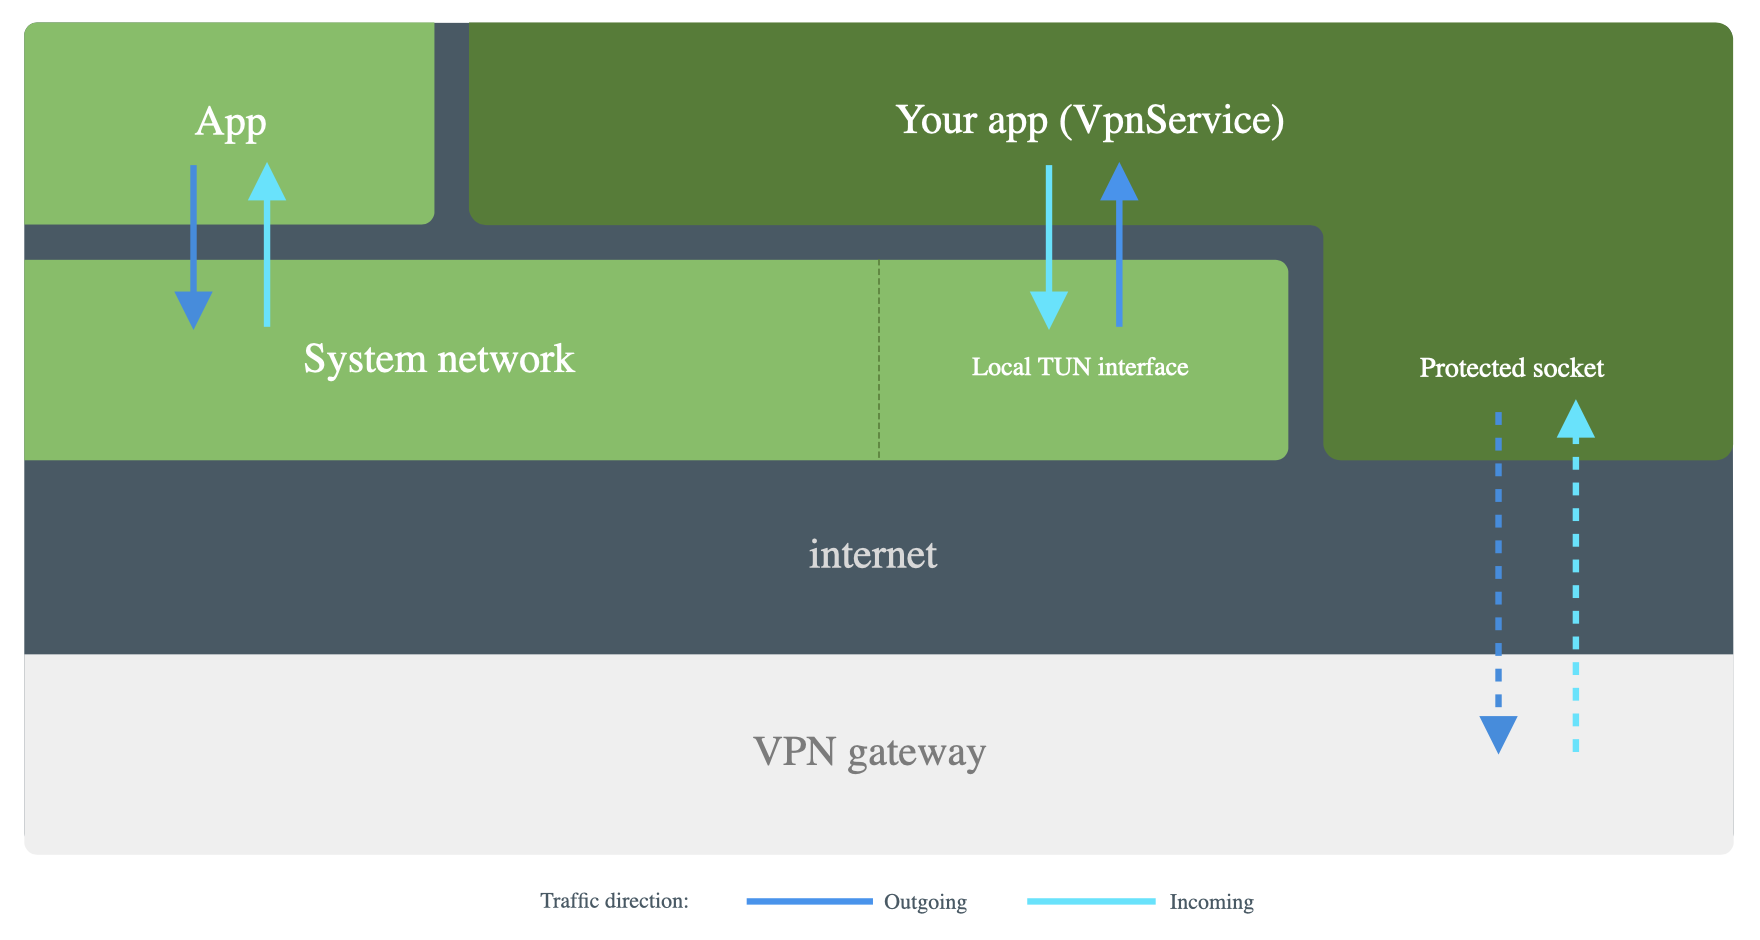
\includegraphics[scale=0.39]{interim_report/interim_graphics/android_vpn}
    \caption{How VpnService connects Android networking to the VPN gateway}
    \label{fig:timeline}
\end{figure}

\vspace{12pt}

%\chapter{Chapter}
%Chapters are in chapters folder. Each chapter is a separate file. All chapters must be referenced in the thesis.tex file. Document should be built pointing the thesis.tex file. Other files do not have document beginning.
%\section{Section}
%This is a section. A title in your chapter. Sections can be further devided in to sub-sections and subsub-sections.
%
%Originally, Balrogs were Maiar that were later persuaded by Melkor before the Awakening of the Elves. Their first dwellings had been Utumno, but after their master's defeat during the War for Sake of the Elves, the Balrogs and other creatures in Melkor's service escaped and went to Angband\footnote{http://lotr.wikia.com/wiki/Angband}.
%\subsection{Sub Section}
%	This is a subsection and they get listed in the TOC(Table Of Content).
%\subsubsection{Sub Sub Section}
%	This is a sub sub section and they do not get listed on TOC.	
%\section{Figures}
%Figures should  be referenced before the actual figure in the text. Figure \ref{bounding} depicts the left side view of the death star. 
%	\begin{figure}[H]
%		\includegraphics[width=8cm]{a.jpg}
%		\centering
%		\caption{Death star, left side view}
%		\label{bounding}
%	\end{figure}
%
%\section{Un-ordered List}
%	
%\begin{itemize}
%	\item Item 1
%	\item Item 2
%	\item Item 3
%	\item Item 4
%	\item Item 5
%\end{itemize}
%
%\section{Ordered List}
%
%\begin{enumerate}
%	\item One item
%	\item Another item
%	\item And another one
%\end{enumerate}
%
%\section{Table}
%Tables should be referenced in the text before the appearance of the table. Table \ref{acc_cross} shows some numbers and by decoding it you prove that the answer for life and everything is 42.
%\begin{table}[H]
%\centering
%\caption{Some numbers with titles}
%\label{acc_cross}
%\vspace{0.4cm}
%\begin{tabular}{|l|l|l|l|l|l|}
%\hline
%\# & Epochs & LR      & Batch size & LSB  & RSB  \\ \hline
%1.1  & 50     & 0.1     & 10         & NA   & NA   \\ \hline
%1.2  & 50     & 0.01    & 10         & 36\% & 31\% \\ \hline
%1.3  & 50     & 0.001   & 10         & 41\% & 36\% \\ \hline
%1.4  & 50     & 0.0001  & 10         & 43\% & 37\% \\ \hline
%1.5  & 50     & 0.00001 & 10         & 40\% & 37\% \\ \hline
%1.6  & 100    & 0.01    & 10         & 38\% & 31\% \\ \hline
%\end{tabular}
%\end{table}
%
%\section{Bibliography}
%Harvard ref style is used here. You can change the style as you prefer. \citep{ban2014} or \citet{ban2014}.